\section{Data}
\par We conducted image classification experiments by using MNIST \cite{lecun-mnisthandwrittendigit-2010} and Fashion-MNIST dataset \cite{xiao2017fashionmnist}. 

\par MNIST is the database of $28\times28$ pixel grayscale images of handwritten digits from 0 to 9. From this dataset, we select the data labeled 0 or 1 for binary classification and make a new dataset. The data 0 have been relabeled as 1 and the data 1 have been relabeled as -1. This dataset consists of 12,665 training images (6,742 images are labeled as 1) and 2,115 evaluation images (1,135 images are labeled as 1). 

\par Fashion-MNIST is the database of $28\times28$ pixel grayscale images of 10 types of fashion products,  T-shirt/top, trouser, pullover, dress, coat, sandal, shirt, sneaker, bag, ankle boot. Labels are assigned from 0 to 9 in this order. From this dataset, we select the data labeled 0 or 1 for binary classification and make a new dataset. The data 0 have been relabeled as 1 and the data 1 have been relabeled as -1. This dataset consists of 12,000 training images (6,000 images are labeled as 1) and 2,000 evaluation images (1,000 images are labeled as 1).

\begin{figure}[htb]
    \centering
    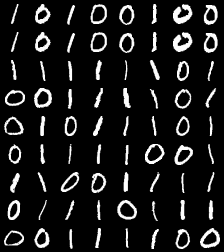
\includegraphics[keepaspectratio, scale=0.5]{experiment/figure/mnist.png}
    \caption{Some images of MNIST labeled with 0 and 1.}
    \label{fig:mnist}
\end{figure}

\begin{figure}[htb]
    \centering
    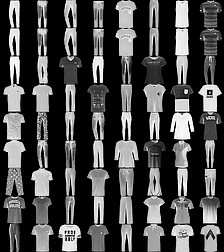
\includegraphics[keepaspectratio, scale=0.5]{experiment/figure/fmnist.png}
    \caption{Some images of Fashion-MNIST labeled with 0 (T-shirt/top) and 1 (trouser).}
    \label{fig:fmnist}
\end{figure}

\par These images have too many pixels, so we reduce them to $8\times8$ pixel images by setting the resize method of the OpenCV library with the interpolation method set to inter\_area \cite{opencv_library}. After that, they are flattened by converting it to a $64$-dimensional vectors and normalized.